\documentclass{standalone}
\usepackage{amsfonts, amsmath, amssymb, bm} %Math fonts and symbols
\usepackage{dcolumn, multirow} % decimal-aligned columns, multi-row cells
\usepackage[colorlinks=true]{hyperref}
\usepackage{graphicx, subfigure, float} % graphics commands
\usepackage[margin=1in]{geometry} % sets page layout
\usepackage{setspace}% allows toggling of double/single-spacing
\usepackage{verbatim}% defines environment for un-evaluated code
\usepackage{natbib}% defines citation commands and environments.
\singlespace % set document spacing to single
\bibpunct[, ]{(}{)}{,}{a}{}{,} % sets the punctuation of the bibliography entires.
\newcolumntype{d}[1]{D{.}{.}{#1}} % defines a decimal-aligned column
\usepackage{tikz}
\usetikzlibrary{intersections}
\usepackage{enumerate}
\usepackage[utf8]{inputenc}
\usepackage[english]{babel}
\hyphenpenalty=10000

\begin{document}
    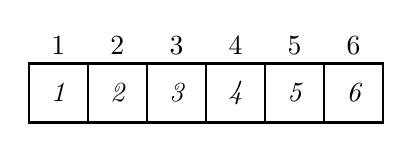
\begin{tikzpicture}[
        list/.style={
            % The shape:
            rectangle,
            % The size:
            minimum size=.75cm,
            % The border
            thick,
            draw=black,
            % The filling
            fill=white,
            % Font
            font=\itshape
        }]

        \foreach \x/\xtext/\xletters in {0/1/1, 0.75/2/2, 1.5/3/3, 2.25/4/4, 3/5/5, 3.75/6/6}
        {
            \node [list]  at (\x,0) {\xletters};
            \node at (\x,.6) {\xtext};
        }
        
    \end{tikzpicture}
\end{document}
